
\chapter{Software, 1960-1980ish}


\section{The Software Crisis}
% \todo{DEC PDP-8 and PDP-11; IBM System/360 and OS/360; Multics; Unix; C}As the 1960s progressed,
% the notion of
% \textit{software} became more established,and the programs being written served the authors to a
% much greater extent.
% Prior to the 1960s, programs were often tailor-made for a specific
% machine. There was no hope of re-using the program on another machine. For most of the users, their
% organization had spent a considerable portion of their budget on their system, and they were
% expected to use it for a long time. Retargetable compilers did not exist.

Note that we will discuss some giants of computing history in this chapter who cast long
shadows over the field; however, we will primarily focus on those involved in the
development of compilers and programming languages.
In particular, we will not do justice to key figures from Bell Labs, such as
Brian Kernighan, Ken Thompson, Dennis Ritchie, Claude Shannon, and Doug McIlroy.
I can recommend \textit{The Idea Factory} for a more comprehensive account.

As Hopper and Backus had put it numerous times, programming was still exceedingly
painful at this point in time, and the relative cost of programming kept increasing.
As machines became cheaper and more powerful, the share of the cost of building and
running a program devoted to programming increased, and thus the importance of
ease of programming increased as well.

Michael Mahoney, doctor history and history of science, goes so far as to describe programming
and computer design in this way as early as 1945
\cite[The Structures of Computation]{the-first-computers-2002}:
\begin{quotation}
	The kinds of computers we have designed since 1945 and the kinds of programs we have written for
	them reflect not the nature of the computer but the purposes and aspirations of the groups of people
	who made those designs and wrote those programs, and the product of their work reflects not the
	history of the computer but the histories of those groups, even as the computer in many
	cases fundamentally redirected the course of those histories.
\end{quotation}

While this description was correct about the \textit{direction} compiler engineering
and programming language design were going, the statement was far too strong to make
about the year 1945.
Automatic programming was still scarcely more than synthetic machine code so the programmer
did not have to concern themselves with the details of the particular machine's instruction set
to the same extent, but they were still very much writing programs by writing specific instructions
instead of concerning themselves with the problem they were trying to solve and allowing the
compiler to turn that into proper machine code.

American historian of computing and aerospace Paul Ceruzzi describes the situation in 1968:

\begin{quotation}
	Despite great strides in software, programming always seemed to be in a state of crisis and
	always seemed to play catch-up to the advances in hardware. This crisis came to a head in 1968, just
	as the integrated circuit and disk storage were making their impact on hardware systems. That year,
	the crisis was explicitly acknowledged in the academic and trade literature and was the subject of a
	NATO-sponsored conference that called further attention to it. Some of the solutions proposed were a
	new discipline of software engineering, more formal techniques of structured programming, and new
	programming languages that would replace the venerable but obsolete COBOL and FORTRAN
	\footnote{Readers may find it entertaining that Ceruzzi describes COBOL and FORTRAN
		as obsolete \textit{by 1968}; both are still heavily used in some industries,
		and one of the very first compilers to adopt MLIR (to be discussed in a later chapter)
		is a Fortran compiler\cite{spickett_flang_levels_up_2025}.}. Although
	not made in response to this crisis, the decision by IBM to sell its software and services separately
	from its hardware probably did even more to address the problem. It led to a commercial software
	industry that needed to produce reliable software in order to survive. The crisis remained, however,
	and became a permanent aspect of computing. Software came of age in 1968; the following decades would
	see further changes and further adaptations to hardware advances.
	\cite{history_of_modern_computing_2003_ceruzzi}
\end{quotation}

Backus describes this as part of the motivation for beginning work on \ftn{}
\cite[\textit{The Economics of Programming}]{hopl_backus_history_of_fortran}:
\begin{quotation}
	Another factor that influenced the development of Fortran was the economics
	of programming in 1954. The cost of programmers associated with a computer
	center was usually at least as great as the cost of the computer itself\dots
	Thus, programming an debugging accounted for as much as three quarters of the
	cost of operating a computer; and obviously, as computers got cheaper, this
	situation would get worse.
\end{quotation}

Thus this chapter is about the efforts to make programming easier and more productive
to address this crisis. Software rose in importance in industry, it became a field of
study in academia, and true research on compilers and programming languages began.










\section{Multics and Unix at Bell Labs}

There is no avoiding Multics and UNIX if we are to discuss the development of compilers at Bell Labs.
We will cover the history of the American Telephone and Telegraph Company (AT\&T)
in \textit{very} broad strokes to contextualize the development of the programming languages
and compiler tools developed in this time period.

In very broad strokes, American Telephone and Telegraph Company (AT\&T) was a government-sanctioned
monopoly that provided telephone service to the United States.
They became a monopoly by buying up smaller telephone companies across the country.
Over time, they found they needed quite a bit of fundamental science in order to keep up with the
requirements of servicing the entire country, so in 1925 they created Bell Telephone
Laboratories in New York. If they did not continue providing quality service, the government could
(and very often did) threaten to break up the company, so this need was existential.

During the second world war, they expanded to New Jersey, early 1960s they moved to Murray Hill,
in suburban New Jersey, where they had a few thousand employees.
The laboratory was responsible solely for research, and thousands of other employees
worked on applying the research and developing the process knowledge needed to bring the
research into the phone system.
This research led to numerous fundamental discoveries and inventions in physics,
materials science and many more domains; these discoveries include the transistor, lasers,
fiber-optics and solar cells, to name a small subset.
Patents were the laboratory's primary measure of success, and they produced many.
At its peak, AT\&T was the nation's largest private employer with over 1 million employees.
If you are interested in an account of Bell Labs in anything close to the proper detail,
I recommend \textit{The Idea Factory} by Jon Gertner; our focus if far too narrow to do
it justice here.

In the early 1960s, the labs spun off a new department, the Computing Sciences Research Center,
off of the mathematics group. This group had about 25 people tasked with software and computing
research, which included operating systems.
In 1961, Fernando Corbat\'{o} at MIT created a timesharing system called CTSS,
or the Compatible Time Sharing System, with relative success.
In 1965 MIT set out to make a successor system with all kinds of enhancements; they partnered with
Bell Labs and General Electric to create the operating system called \textit{Multics}.
The machine was developed at GE (Multics required a special machine), Multics was designed at MIT,
and Bell Labs was responsible for large parts of the software development,
which was primarily done in IBM's PL/I programming language.
Ken Thompson described it as "monstrously over-engineered" and "typical second-system syndrome"
\cite{kernighan_interviews_thompson_2019};
while they had a wonderful time-sharing system in CTSS, they got too ambitious with thier sophomore project.
Ultimately, this project ran long past deadlines and was slow to run and altogether not what
the labs was hoping for, so in 1969 they pulled out of the project.
Honeywell took over Bell Labs' share of the project.

This left a bad taste in their mouths, and Bell Labs leadership sought to avoid operating
systems work in the wake of this venture.
Some of the members of the Multics team had other ideas; they had gotten a taste for
operating systems work, and now they had not operating system to work \textit{on}.
These included Ken Thompson, Dennis Ritchie, and Doug McIlroy.

At the time, Ken Thompson was researching file systems on an outdated and underused
Digital Equipment Corporation (DEC) PDP-7 machine from the acoustics group.
\footnote{Because acoustics research was so core to Bell Labs' and AT\&T's mission,
that department got just about anything they asked for in terms of computing resources,
hence the outdated PDP-7 sat unused in their offices--they already had more powerful machines.}
He originally just used it for writing video games, until finally getting around to
his research on file systems.
He developed disc scheduling algorithms to maximize throughput on the PDP-7's disc drive.
To adequately test the performance of his file system algorithms, he needed some test
programs to stress the file system.
At some point in this process, he realized he was not far off from an
operating system of his own\cite{kernighan_interviews_thompson_2019}:

\begin{quotation}
At some point, I realized with out knowing it up until that point, that I was 
three weeks from operating system, with three programs, one a week. I needed an 
editor to write code, I needed an assembler to turn the code into language I 
could run, and I needed a kernel overlay, call it an operating system.  
Luckily, right at that moment, my wife went on a three-week vacation to take my 
one-year-old to visit her parents in California. One week, one week, one week, 
and we had Unix.
\end{quotation}

Thompson's assembler was not a complete toolchain; there were no libraries, linkers, or loaders.
The entire assembly program had to be presented to the assembler all at once,
and the output was directly executable. Thus the \texttt{a.out} naming convention for
the default executable output of modern compilers was born (\textit{a}ssembly \textit{out}put).
Even after the system gained more toolchain components, the name remained.

Very early on, Thompson's system picked up very impressive users.
Two at a time, Dennis Ritchie, Doug McIlroy, Morris McMahon, and Brain Kernighan
all became users on Thompson's new system.
They sent a proposal to get a PDP-10, which was top-of-the-line at the time,
to port Unix to a more powerful machine.
This was rejected as soon as Labs leadership saw it was related to operating systems,
in spite of the fact that their request was well within budget.
Joe Ossanna (another colleague) came up with a proposal that
positioned their need for a PDP-10 as a research project to develop better typesetting
software for filing patent applications (notably missing any mention of operating
systems).
Ossanna developed the Nroff and Troff typesetting programs to fullfil their claimed
goal of helping the patent office.
The patent office loved their software, and they ended up buying the computing group
a PDP-11\footnote{While many resources will mention the PDP-11, they usually refer to the
PDP-11\textit{/22}; very few of original PDP-11s (which the computing center worked on)
were ever produced, but the refreshed models had many users.} sometime in the early 1970s.
Unix came up on the PDP-11 almost immediately.
Thus we have the basis for discussing the subsequent development of compilers
and programming languages at Bell Labs.


\subsection{Personal Histories}

The following sections will feature many of the same figures;
here we will introduce them so their interleaving stories may be told
uninterrupted in the following sections.
Readers unfamiliar with the history of Unix may find unfamiliar terms in these
personal accounts; these will be discussed in the following sections after
our characters have been introduced.

\subsubsection{Doug McIlroy, Joined 1958}

Douglas McIlroy was born in Fishkill, New York.
His father worked in electrical engineering and spent time at
MIT and ended his career at Cornel, having contributed to the RADAR effort in World War II.
His father collected maps, and Doug grew an interest in maps himself.
One day, while ill in bed with chicken pox, his father assigned him the task of drawing
a dam on a USGS map, and showing which regions would be inundated by the dam
\cite{doug_mcilroy_oral_history_2019}.
His mother, too, had a master's degree in physics from the University of Rochester,
which was very unusual at the time. She was forced to audit some of her classes there,
because "women can't take this class! But you can sit in on it, if you want."
Thus he was raised in an engineering-minded household.

Barbara, his wife, also studied mathematics and faced discouragement similar to his mother's.
They ended up meeting at the laboratory, where Doug recalled that some figures at the labs sought
to improve the situation for women, specifically Bernie Holbrook.

Doug joined Bell Labs in 1958 and shortly thereafter earned his
PhD in applied mathematics from MIT.
McIlroy became head of the Computing Techniques Research department in 1965, and he's regarded
as one of the most brilliant members of the staff by key members that readers may be more familiar with.

He is described by nearly everyone at the Bell Labs Computing Research Center
(who wrote or spoke about their time there)
as the most brilliant member of that team that no one has heard of
\cite{kernighan_interviews_thompson_2019}; Ken Thompson described him as
"the smartest one of all of us and the least remembered or written down of all of us."

He was relatively hands-off as a manager, preferring to peek into his employees' offices
with suggestions or interesting problems and wait for the employees to let \textit{him} know
what needed to be done, rather than assigning tasks directly.
His employees respected his tasted in technical and personal matters,
as Brian Kernighan describes\cite{kernighan_unix:_2020}:

\begin{quotation}
	Unix might not have existed, and certainly
	would not have been as successful, without Doug's good taste and sound
	judgment of both technical matters and people.
\end{quotation}

\begin{figure}
	\centering
	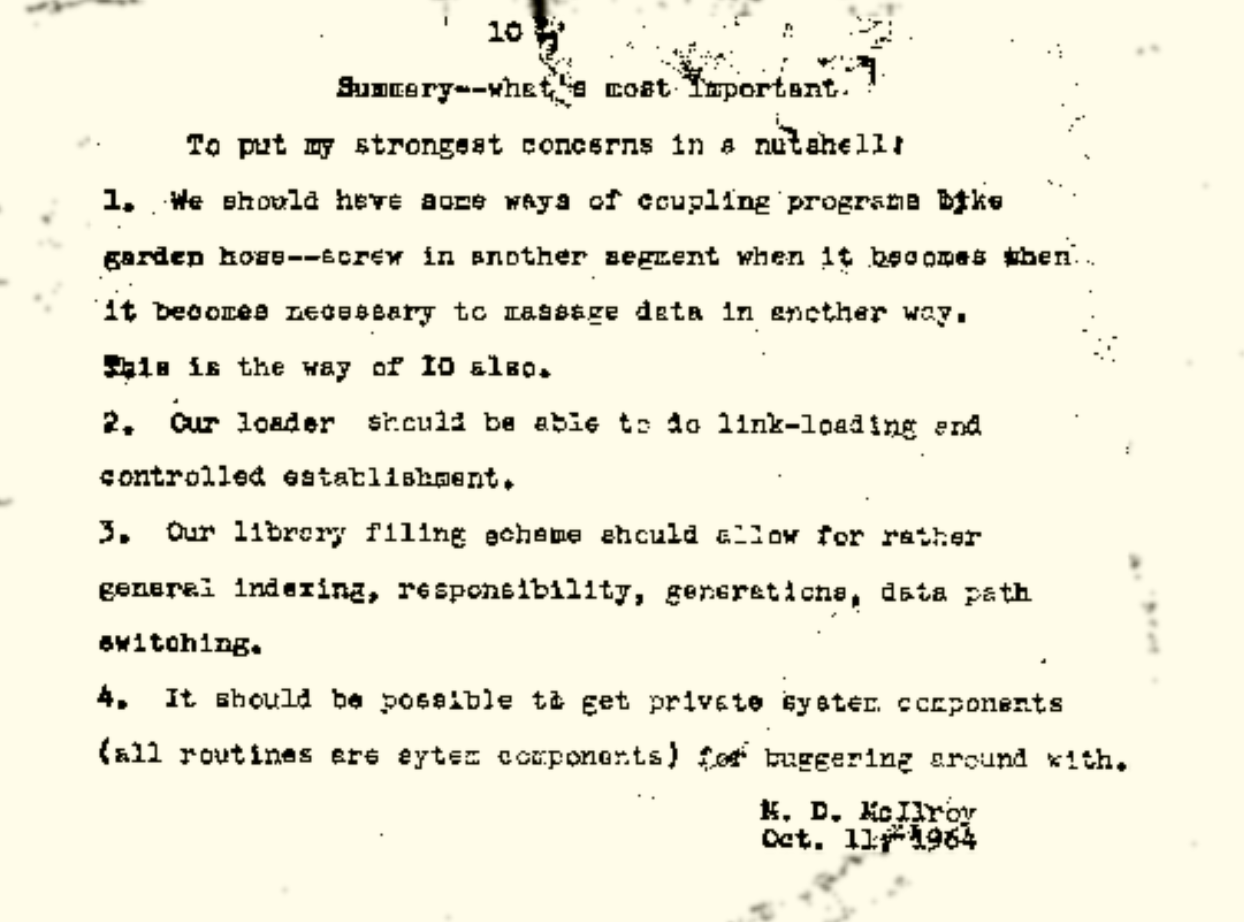
\includegraphics[width=0.7\textwidth]{resource/software/unix/doug-1964-pipes.png}
	\caption{Doug McIlroy's 1964 memo proposing Unix pipes\cite{doug_mcilroy_origin_of_unix_pipes_1964}.}
	\label{fig:unix-pipes-mcilroy-memo}
\end{figure}

In 1964, he circulated a memo which led to Unix pipes\cite{doug_mcilroy_origin_of_unix_pipes_1964}
(see \ref{fig:unix-pipes-mcilroy-memo}) though it took him quite a while to convince
Ken Thompson that he really ought to implement them.
Aside from pipes, he wrote many common Unix utilites we still use today, like
\texttt{diff}, \texttt{sort}, \texttt{join}, \texttt{tr}, \texttt{echo}, \texttt{tee}, and \texttt{spell}.

He hired Alfred Aho in 1967\cite{aho_oral_history_2022}:

\begin{quotation}
	I was interviewed by a department head by the name of Doug McIlroy. He was an applied
	mathematician from MIT. He had been at Bell Labs for a few years before me. Amongst other things, he
	had co-invented macros for programming languages and he's also in this class of one of the smartest
	people I've ever met.
\end{quotation}

\subsubsection{Ken Thompson, Joined 1966}

\todo{Ken's oral history is rich and includes fun stories about how he was recruited to the labs.}

\subsubsection{Dennis Ritchie, Joined 1967}


\subsubsection{Jeffrey Ullman, Joined 1967}

\todo{This section can be shorter since Ullman went back to Princeton and only consulted at the lab part-time.}

\subsubsection{Alfred Aho, Joined 1967}

Alfred grew up in a Finnish household, and when he showed up to Kindergarten,
he couldn't speak any English.
In his first report card, the teacher told his parents that "Al can't speak any English!",
and in the next report card, the teacher said reported that "Al speaks \textit{too much} English!";
so he learned it relatively late and became quite a social kid.
Alfred played music all throughout his childhood, and the schools he went to
as a kid had quite good musical programs.
He went to University of Toronto for undergraduate school and continued playing
the violin all through his years at Bell Labs. He was an only child. He had a
proclivity not only for music but for mathematics and reading science fiction.

After finishing his undergraduate degree in Toronto in engineering physics,
he got a masters and then PhD
from Princeton University in electrical engineering and computer science,
completing the latter in 1967.
At Princeton took a course from John Hopcroft on computer science theory with a heavy emphasis on
automata and language theory, which sparked his long-lasting interest in formal languages.
His PhD thesis was on extending the theory of context-free grammars, an area of
expertise that would serve him well at the Labs.

One of the fist people he met at Princeton was Jeffrey Ullman, who had also recently
started there, beginning a long-term friendship and collaboration between the two
\cite{aho_oral_history_2022}:

\begin{quotation}
	One of the first people that I met at Princeton was a Columbia graduate by the name of Jeffrey
	Ullman. He had just gotten his undergraduate degree from Columbia University and also had come to
	study digital systems in the EE department at Princeton. So, he and I became close friends. When we
	graduated from Princeton, we both joined the newly formed Computing Sciences Research Center at Bell
	Labs. There we developed a lifelong collaboration on subjects ranging from algorithms, programming
	languages, to the very foundations of computer science. I was very fortunate to have met some of the
	greatest people in the field and to have gotten to know them and work with them.
\end{quotation}

His PhD advisor was John Hopcroft, whom he would also continue to work with for a long time.
He told Alfred to "find his own research problem," and he turned to his interest in
programming languages and compilers.
He was always very keen on precision; he wanted to use precise terms and he would
press even his own friends to be very precise in their informal discussions, and
this acuity for precision extended to his thesis, which was on the very precise
understanding of the \textit{syntax} and the \textit{semantics} of programming languages.
Alfred would contribute his deep understanding of the theory of automata and programming
languages to the Labs, where there were many other brilliant people who were more practical
and lacked familiarity with the literature.
In 1967 his good friend Jeffrey Ullman had started working at Bell Labs, and a few months
after starting there, Alfred interviewed there.
He was interviewed by Doug McIlroy, who hired him.
For some time, he and Jeffrey worked together at the Labs, but Jeffrey had wanted to
spend more time in academia than Alfred, so he returned to Princeton's electrical
engineering department, but continued to consult at Bell Labs one day a week.
Thus the two continued to work together.
Alfred described their collaboration at Bell Labs:

\begin{quotation}
	He stayed at Bell Labs for a few years and went to Princeton University where he
	joined the faculty of the electrical engineering department, but he would come and spend one day a
	week consulting at Bell Labs. His consulting stint, he would come Fridays and sit in my office
	all day. The conversations that we'd have would range over all sorts of topics, and sometimes he'd
	mentioned that he was working on a problem with a colleague at Princeton, and after describing the
	problem, I might say, "You're kidding," and he said, "Oh, you're right. The solution is obvious,
	isn't it?" I don't know whether I would say dynamic programming or whatever, but several papers
	came out of this intense collaboration, and we got to the point where we could communicate with just
	a few words. We had a very large, shared symbol table.
	\cite{aho_oral_history_2022}
\end{quotation}

Ken Thompson joined the labs several months before the two of them to
start working on Multics, and had developed a plethora of tools based on
regular expressions, such as \texttt{grep}.
This combined with the \texttt{ED} and \texttt{QED} editors that came from MIT
and were shipped with Multics sparked Alfred's interest in regular expressions.

Aho is probably best known for the textbooks he co-authored with his friend Jeffrey,
colloquially known as \textit{The Dragon Book} (\citetitlecite{the_dragon_book_aho_ullman_sethi_1986})
and his book with John Hopcroft on algorithms, \citetitlecite{aho_hopcroft_algorithms_1974}.

\subsubsection{Brian Kernighan, Joined 1969}

\subsubsection{David McQueen, Joined 1981}

David didn't start working at the labs until much later than the others in this section
and he primarily worked on his own, unlike the others mentioned in this section.
Because of his work on Meta Language and type theory, we include some of his personal history here
as well.


\section{The First Unix Compilers}

Alfred Aho described this era of compiler history
as as cambrian explosion of programming languages and compiler tools
\cite{aho_bell_labs_role_in_programming_languages_2025},
and there were several reasons for that.
Tools were developed that made the description of compiler front-end
tools extremely simple, the computing center got access to machines with
more memory, and the theory of parsing context-free grammars advanced.
The Labs employees worked all of these together to produce many compiler
tools.

While Doug was the department head of the Computing Sciences Research Center,
he would regularly stop into the offices of his employees and drop ideas and requests
to them. In one case, he mentioned to Ken how convenient it would be to have
a tool for searching text files for patterns.
Ken already had a rough version of such a tool in his home directory,
so the next day he showed Doug his program and thus was born \texttt{grep};
many such tools came to be like this.

On another similar occasion, Doug walked into Ken's office to discuss the TMG language
(standing for TransMoGrifier),
designed by Robert McClure\cite{mcclure_tmg_compiler_compiler_1965}, one of his friends at the lab.
McClure had gotten defensive about this language, and when he left the lab,
he claimed it was proprietary and nobody else could use it.
TMG was a top-down recursive-descent compiler-compiler for context-free grammars
and procedural elements similar to Yacc, a tool to help write compiler
front-ends.
See this example from Doug's TMG manual\cite{tmg_manual_mcilroy_1972}
and notice the similarities to modern parser generators and Backus-Naur Form:

\begin{quotation}
This simple program defines the translation of fully parenthesized infix 
expressions to Polish postfix for a stack machine.
\begin{lstlisting}[frame=single]
    expr: <(>/exp1 expr operator expr <)> = { 3 1 2 };
    exp1: ident = { < LOAD > 1 };
    operator:
    op0: <+>/op1 = { < ADD > };
    op1: <->/op2 = { < SUB > };
    op2: <*>/op3 = { < MPY > };
    op3: </>     = { < DIV > };
\end{lstlisting}
\end{quotation}

Ken recounts\cite{kernighan_interviews_thompson_2019}
the story of how Doug brought a full TMG compiler \textit{written in TMG,
on paper} to Ken's office. He then decided to feed the TMG program into his TMG compiler
\textit{by hand} to produce an assembly listing of the TMG program.
He then went over to Ken's keyboard and typed in the program that his TMG-TMG compiler
had produced, and with astonishingly few errors, they had a working TMG compiler on the PDP-7.

Ken's logical next step was to use this new TMG compiler to
write a \ftn{} compiler for the PDP-7 because
"no computer was complete without \ftn{}."
Now, the PDP-7 was only 8k of 18-bit words of memory and Ken's Unix system needed
about half of that just to run, leaving only 4k for user programs.
Once completed, the new \ftn{} compiler took far more memory than was available for
user programs, so he had to cut down the TMG program to get a program small enough to
fit on the machine but capable enough to facilitate a usable programming language.
Once he finally cut down his compiler to 4k, he called that programming language \textit{B}.
His ill-fated attempt at producing a \ftn{} compiler ended up being a very different language,
based more so on BCPL than on \ftn{}
\footnote{The origins are really unclear. Ken himself mentions \ftn{} as his only inspiration
for B in a live interview\cite{kernighan_interviews_thompson_2019},
however Dennis Ritchie describes it as a "language of his own" and
"BCPL squeezed into 8K bytes of memory and filtered through Thompson's brain"
\cite{development_of_c_language_chist_ritchie_1996}.
He describes the name as either a contraction of BCPL or (less likely) a contraction
of Bon, a language Thompson developed for Multics.}.
BCPL had been designed by Martin Richards at MIT in the mid-1960s, and thus had found
its way onto MIT's CTSS system, which Bell Labs employees were familiar with.

\section{BCPL and B}

BCPL, B and C may differ syntactically, but semantically they are very similar
and operate at a similar level of abstraction.
The BCPL compiler was allowed to use more memory than Thompson had on the PDP-7,
so it allowed for more complicated expression-oriented language features.
Dennis Ritchie points out the following two examples as only being possible
in BCPL and not in B or C due to memory constraints
\cite{development_of_c_language_chist_ritchie_1996}:

\begin{lstlisting}[language=c,frame=single]
let P1 be (*@\textbfit{procedure}@*)
and P2 be (*@\textbfit{procedure}@*)
and P3 be (*@\textbfit{procedure}@*)

E1 := valof ( (*@\textbfit{declarations}@*) ;
              (*@\textbfit{commands}@*) ;
              resultis E2 ) + 1
\end{lstlisting}

Because the entire program was held in memory, the BCPL compiler could make
procedure \textbfit{P3} available to expressions inside procedure \textbfit{P1},
but the B compiler was limited to a one-pass technique and could not provide such features.
On the other hand, some BCPL features were purposefully left out of B; for example,
to share data between separately compiled source files, BCPL programs had to use
a global buffer. To make a procedure or variable available to other source files,
the programmer had to manually associate the name with an offset into this buffer,
similar to the \texttt{COMMON} block in \ftn{} programs.
In more mature B compilers and later in C, the linker handles this automatically.

\begin{figure}[h]
    \centering
    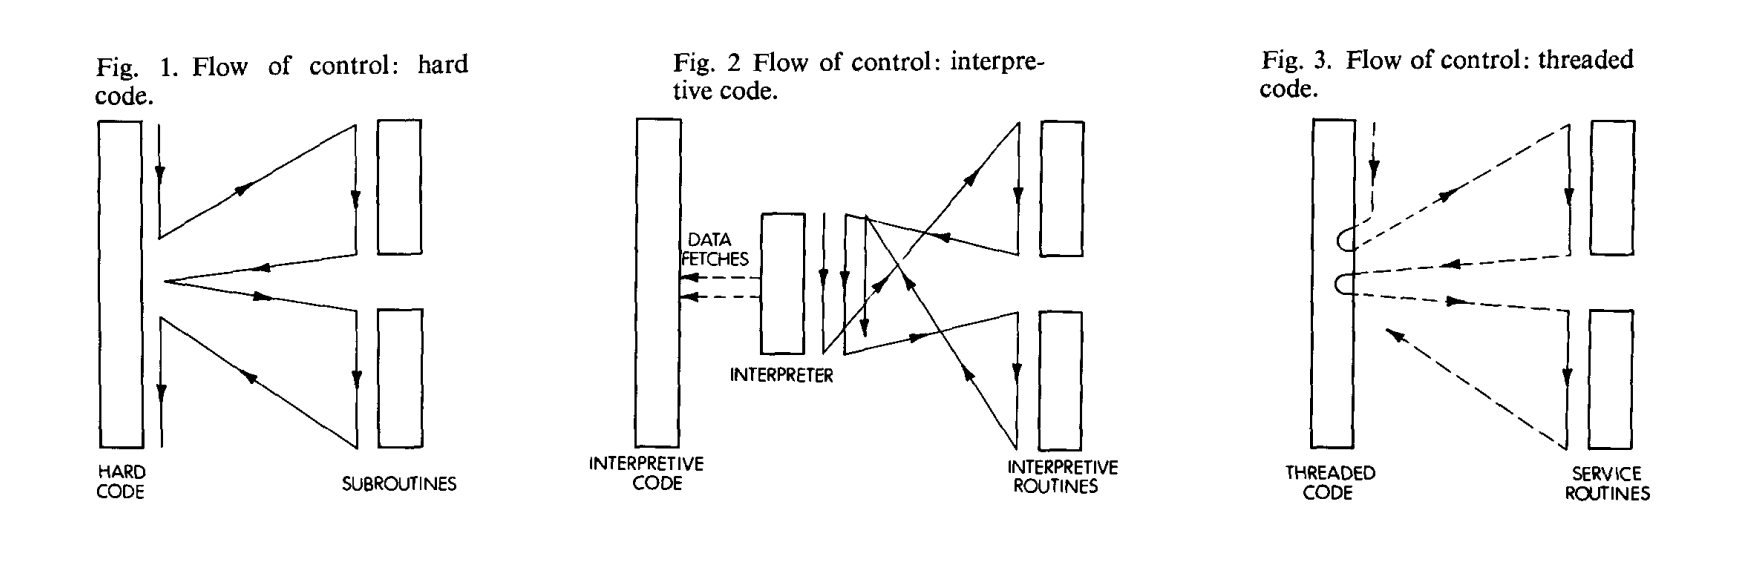
\includegraphics[width=0.8\textwidth]{resource/software/unix/bell-threaded-code-figures.png}
    \caption{Execution of Threaded Code\cite{bell_threaded_code_1973}}
    \label{fig:bell-threaded-code}
\end{figure}

The B compiler did not emit machine code directly, but instead used
\textit{threaded code}\cite{bell_threaded_code_1973}, an early form of \gls{bytecode}
operating on a simple stack machine, which was then interpreted.
James Bell claimed that this threaded code needed no interpreter,
but really, the execution model for threaded code is just a specification
for an interpreter without outside the routines responsible for executing a given
bytecode instruction.
Today this would be considered a bytecode interpreter, but in the day when interpreters
were only known to interpret the source language directly, his ideas may have seemed
distinct from other forms of interpretation.
See Bell's depiction of the execution of threaded code \ref{fig:bell-threaded-code}.

Neither B nor BCPL had types; only the addressable size of data for the particular machine.
Since pointers were just integers representing offsets into memory, pointer arithmetic
was natural in both languages, and both had syntax sugar to facilitate pointer arithmetic
and dereferencing of offsets into arrays.

\begin{lstlisting}[language=c,frame=singl]
/* Declaring an array of 10 integers */
let V = vec 10 /* BCPL */
auto V[10];    /* B    */

/* Accessing element i of array V */
V!i            /* BCPL */
*(V+i)         /* B    */
V[i]           /* B    */
\end{lstlisting}

After Ken had the TMG version of B working, he \gls{bootstrap}ped the compiler
by implemented it in B.
Dennis Ritchie recalls\cite{development_of_c_language_chist_ritchie_1996}:

\begin{quotation}
During development, he continually struggled against memory limitations: each 
language addition inflated the compiler so it could barely fit, but each 
rewrite taking advantage of the feature reduced its size. For example, B 
introduced generalized assignment operators, using x=+y to add y to x. The 
notation came from Algol 68 via McIlroy, who had incorporated 
it into his version of TMG.
\end{quotation}

Dennis also recalls this about their language design and implementation decisions:

\begin{quotation}
Although we entertained occasional thoughts about implementing one of the major 
languages of the time like Fortran, PL/I, or Algol 68, such a project seemed 
hopelessly large for our resources: much simpler and smaller tools were called 
for. All these languages influenced our work, but it was more fun to do things 
on our own.
\end{quotation}

By 1970, the team had been able to acquire the PDP-11, which they promptly ported Unix to,
along with the B \gls{bytecode} interpreter and a small assembler written in B.
As the number of PDP-11 users grew, so too did their B codebase, which now included
quite a few programs and subroutines, as a result of the tedium of writing assembly,
which was the only alternative.
B proved useful--however, the new machine revealed some serious inadequacies.
The only data type in BCPL and B was the \texttt{cell}, roughly equivalent to the hardware's
machine word.
The 18-bit PDP-7\footnote{18-bit might seem like an odd choice to the modern reader;
most mainframe computers had 36-bit words, and the PDP-7 was marketed as a smaller system.
Thus at 18-bits, it would be marketed as roughly half a mainframe.}
did not map cleanly to the 16-bit PDP-11.
BCPL on the PDP-7 had support for floating-point operations through special operators, but this
only worked because the floats could fit in a single word and this was not possible on the PDP-11.

\begin{quotation}
For all these reasons, it seemed that a typing scheme was necessary to cope 
with characters and byte addressing, and to prepare for the coming 
floating-point hardware. Other issues, particularly type safety and interface 
checking, did not seem as important then as they became later.
Aside from the problems with the language itself, the B compiler's 
threaded-code technique yielded programs so much slower than their 
assembly-language counterparts that we discounted the possibility of recoding 
the operating system or its central utilities in B.
\cite{development_of_c_language_chist_ritchie_1996}
\end{quotation}

In 1971, Dennis Ritchie began extending B by adding a character type and directly generating
PDP-11 machine code.
Thus the creation of a compiler capable of generating efficient machine code on a system with
very little memory and the transition from B to C were simultaneous.
Dennis renamed the B compiler to \texttt{NB}, or \textit{New-B}, and then \textit{C}
shortly thereafter.

\section{C}

Dennis's new language now had types and new addressing schemes, and it evolved quickly.
\textit{New-B} existed so briefly that no full description of its syntax or semantics was
ever written.

The run-time overhead associated with BCPL and B's vector indexing semantics were
addressed in C:

\begin{quotation}
Values stored in the cells bound to array and pointer names were the machine 
addresses, measured in bytes, of the corresponding storage area. Therefore, 
indirection through a pointer implied no run-time overhead to scale the pointer 
from word to byte offset. On the other hand, the machine code for array 
subscripting and pointer arithmetic now depended on the type of the array or 
the pointer: to compute \texttt{iarray[i]} or \texttt{ipointer+i} implied 
scaling the addend \texttt{i} by the size of the object referred to.
\cite{development_of_c_language_chist_ritchie_1996}
\end{quotation}

C gained a type system, overlaying semantics onto the raw bits that BCPL and B users
were working with.
The type system was heavily inspired by ALGOL 68, though not necessarily in a way the
authors of the ALGOL language would have been happy with, as Dennis himself admits
\cite{development_of_c_language_chist_ritchie_1996}.
Many features were added to the language in a short time; some of the warts that persist in
even modern C were because of Dennis's desire to make porting programs from B to C as 
simple as possible.

For example, the precedence of \texttt{&} and \texttt{==} were made equal in C,
thereby requiring parentheses in the second expression below:

\begin{lstlisting}[language=c,frame=single]
if (a == b & c) { /* ... */ }
if ((c & b) == a) { /* ... */ }
/*  ^ Parentheses required here */
\end{lstlisting}

While many features were added to C in 1972-1973, the preprocessor was likely the most
significant. Dennis implemented it partly at the request of Alan Snyder
(who had also suggested that Dennis add the \texttt{&&} and \texttt{||} to make
boolean logic more explicit) at MIT
in \citetitle{snyder_portable_compiler_for_c_1975}, and
partly inspired by the textual inclusion mechanisms in PL/I and BCPL.
The first version could only \texttt{#include} other files and do simple textual
substitution, though it was soon extended by Mike Lesk and John Reiser to handle macros
with arguments and support conditional compilation.

In the summer of 1973, the language and compiler were mature enough that the team was able
to rewrite the Unix kernel in C.
Ken Thompson had tried once before to port Unix to C, but the language did not support
structures at the time, making the task too onerous to continue.
The compiler was also ported to the Honeywell 635 and IBM 360 and 370, and commonly used
procedures coalesced into what eventually became the standard library.
The first of these major library components was Mike Lesk's input/output library, which
became the basis of the C \textit{standard I/O}.
Dennis and Brian Kernighan wrote the seminal \citetitlecite{the_c_programming_language_1ed_ritchie_kernighan_1989}.
Brian wrote most of the exposition and Dennis wrote most of the programs.
This would come to be common; Brian's gift for technical writing that was easy to understand
made him a common author of documentation and publications.

\section{Aho and Ullman}

\todo{Software (and compilers!) starts to become a real discipline!Ullman was older and further 
along than Aho, and Hopcraft came to Princeton and became Aho's advisor.}

\todo{Ratfor, AMPL, other Kernighan languages.}
\todo{continue with typesetting...}
\section{The Dragon Book}
\begin{quotation}
    Jeff had bought into this idea that it's good for your career to write a 
book about what you're working on. In the '70s, with all this work on Unix and 
C, there was a lot of interest in creating new programming languages and 
compilers. As with the algorithms book, what we did was we performed research 
on efficient algorithms for parsing and for some of the other phases of 
compilation, wrote papers on those  and presented them at conferences. But we 
took the important ideas that we developed and the community had developed over 
several decades and codified them into what are now called the dragon books. The 
first dragon book was published in 1977.We did have theorems and proofs in the 
book, and Jeff had this brilliant idea that the book should have a cover with a 
fierce dragon on it representing the complexity of compiler design,and then a 
knight in armor with a lance. The armor and the lance were emblazoned with 
techniques from formal language theory and compiler theory to slay the 
complexity of compiler design
\dots
In the 1980s, more was known about how to construct efficient compilers. We 
invited Ravi Sethi as a third coauthor, he was at Bell Labs at the time, to join 
us in creating the second version of the dragon book. In the first version, the 
dragon was in red. This second version, the dragon was-- sorry. In the first 
version it was in green. In the second version the dragon was in red. What was 
interesting about the red dragon book was there was a movie that was created in 
1995 titled Hackers with a young Angelina Jolie in it, and in the movie, there 
is the uber hacker that's explaining to the new hackers what you have to read to 
become an uber hacker. He shows them 10 papers and books that you must read, and 
one of them was the red dragon book. When my two children saw this movie, and 
they had seen the red dragon book at home, this is the first time they thought 
their old man was really something because he had one of his books in a 
Hollywood movie. It shows what you have to do to impress your kids these days. 
The red dragon book was 800 pages. In2007, we invited Monica Lam as a fourth 
coauthor to create a third version of the dragon book that had a purple dragon 
on the cover and it was close to a thousand pages. None of us had the heart to 
write a fourth book at this point because it just shows how much new knowledge 
had been created in the area of programming languages and compilers and their 
translators, and we continued to do research in this area to keep up with it.
\cite{aho_oral_history_2022}
\end{quotation}
\todo{Bjarne Stroustrup, C++ (1979); Dennis Ritchie, C (1972); Ken Thompson, B (1969); Brian 
Kernighan, AWK (1977), AMPL (1976), co-author of The C Programming Language (1978)}


\section{The Next 700 Programming Languages}

Published in \citeyear{landin_next_700_prog_langs_1966},
Peter Landin's seminal paper \citetitlecite{landin_next_700_prog_langs_1966} lays out his vision for
the future of programming language design, emphasizing the importance of the programmer's intent
uncluttered by details of the hardware.
He argued that the programmer ought to only consider their intent, and the compiler ought to
consider the operations that would be needed to carry out their intent.

The paper describes a new programming language called IYSWIM, for \textit{If You See What I Mean}.
\todo{type systems, type inference, Hindley Milner, SML.}
\todo{similar vein to Laning and Zierler's algebraic compiler.}

\section{Seymore Cray}
\begin{quotation}
	The CDC 160 and the Origins of the Minicomputer

	The Whirlwind (a computer prototype built at
	MIT) had a word length of only 16 bits, but the story of commercial minicomputers really begins with
	an inventor associated with very large computers: Seymour Cray. While at UNIVAC Cray worked on the
	Navy Tactical Data System (NTDS), a computer designed for navy ships and one of the first
	transistorized machines produced in quantity. Around 1960 Control Data, the company founded in 1957
	that Cray joined, introduced its model 1604, a large computer intended for scientific customers.
	Shortly thereafter CDC introduced the 160, designed
	\cite{nothing_new_since_von_neumann_2000}
\end{quotation}

\section{The DEC VAX and the IBM System/360}
\begin{quotation}
	Through the 1980s the dominant mainframe architecture continues to be a descendent of the IBM
	System/360, while the dominant mini was the DEC VAX, which evolved as a 32 bit extension of the
	16-bit PDP-11.
	\cite{nothing_new_since_von_neumann_2000}
\end{quotation}
\section{Commodification}
\todo{Bill Gates and Paul Allen (Microsoft) | Microsoft BASIC (1975) |
	Developed the first critical piece of commercial software for personal
	computers,establishing the doctrine that software should be a purchased,
	proprietarycommodity. Sun microsystems, each part of the company needed to sell
	to all the others,reason why their compiler was paid; proprietary Unix;}
\pagebreak
\section{Timeline}
\begin{figure}[h]
\begin{luacode}
    local start = 1965
    local _end = 1980
    timeline.draw_timeline({    
        start_year = start,    
        end_year = _end,    
        marker_interval = 5,    
        show_year = false,    
        line_always = true,    
        events = {        
        {1967, "Aho joins Bell Labs shortly after Ullman"},        
        {1972, "C"},        
        {1977, "Brian Kernighan, AWK",delta=-.5},        
        {1977, "The Dragon Book first published",delta=.5},        
        {1979, "Bjarne, C++"},    },})
tex.sprint(string.format("\\caption{TBD, %d--%d}", start, _end))
\end{luacode}
\label{fig:tbd-timeline}
\end{figure}

